\begin{figure}[h]
	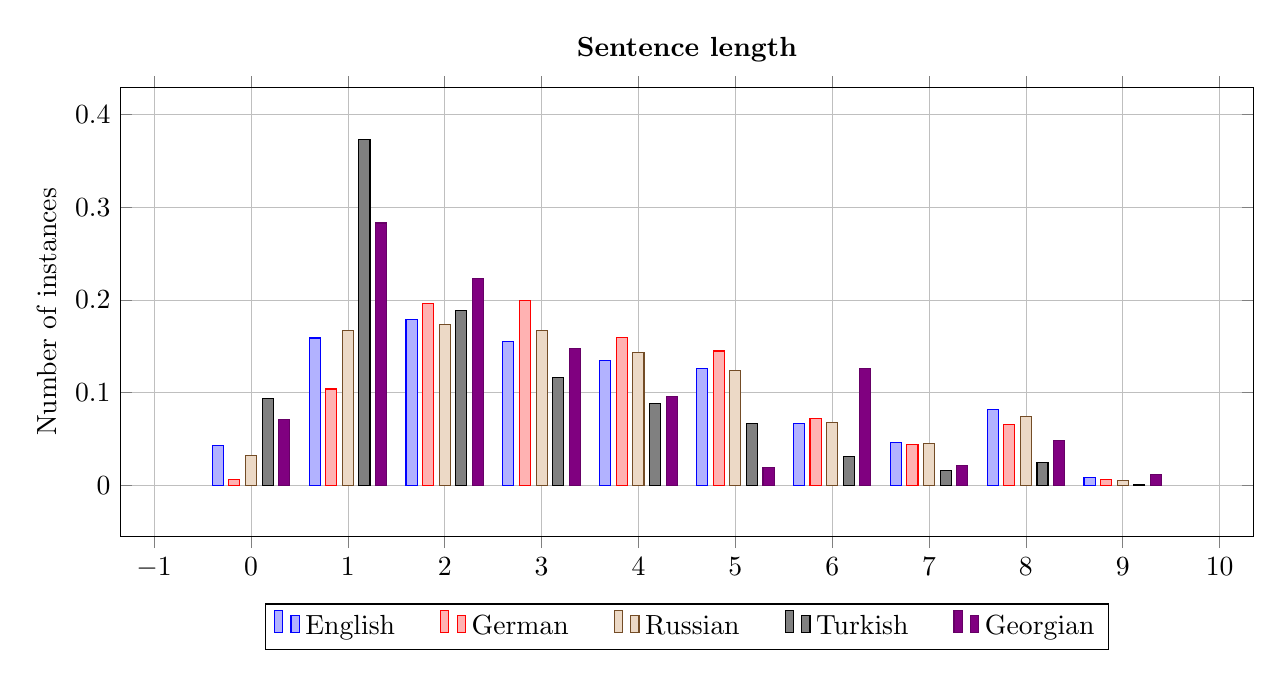
\begin{tikzpicture}
		\begin{axis}[
			ybar,
			x tick label style={/pgf/number format/1000 sep=},
			ylabel=Number of instances,
			enlargelimits=0.15,
			bar width=4pt,
			legend style={at={(0.5,-0.15)},anchor=north,legend columns=-1,/tikz/every even column/.append style={column sep=0.5cm}},
			grid=both,
    			grid style={line width=.1pt, draw=gray!10},
    			major grid style={line width=.2pt,draw=gray!50},
			x=35,
			title=\textbf{Sentence length}
		]

			\addplot coordinates {(0, 0.043) (1, 0.159) (2, 0.179) (3, 0.155) (4, 0.135)
				(5, 0.126) (6, 0.067) (7, 0.046) (8, 0.082) (9, 0.009)};
			\addplot coordinates {(0, 0.006) (1, 0.104) (2, 0.196) (3, 0.199) (4, 0.160)
				(5, 0.145) (6, 0.072) (7, 0.044) (8, 0.066) (9, 0.006)};
			\addplot coordinates {(0, 0.032) (1, 0.167) (2, 0.174) (3, 0.167) (4, 0.143)
				(5, 0.124) (6, 0.068) (7, 0.045) (8, 0.074) (9, 0.005)};
			\addplot coordinates {(0, 0.094) (1, 0.373) (2, 0.189) (3, 0.116) (4, 0.088)
				(5, 0.067) (6, 0.031) (7, 0.016) (8, 0.025) (9, 0.001)};
			\addplot coordinates {(0, 0.071) (1, 0.283) (2, 0.223) (3, 0.148) (4, 0.096)
				(5, 0.019) (6, 0.126) (7, 0.021) (8, 0.048) (9, 0.012)};
            		\legend{English, German, Russian, Turkish, Georgian}

		\end{axis}
	\end{tikzpicture}
	\caption[Sentence distribution by the number of words]{The bar plots depict the sentence distribution by the number of words. As can be seen in the visualization, short to medium-sized sentences (bins 1, 2 and 3) form the majority across all languages. German sentences tend to be longer on average compared to the other languages considered.}
	\label{fig:sent_len_class_distribution}
\end{figure}